\documentclass[12pt,a4paper]{article}
\usepackage{lipsum}
\usepackage[T1]{fontenc}
\usepackage[utf8]{inputenc}
\usepackage[noadjust]{cite}
\usepackage{authblk}
\usepackage[top=2cm, bottom=2cm, left=2cm, right=2cm]{geometry}
\usepackage{fancyhdr}
\usepackage{listings}
\usepackage{csquotes}
\usepackage{color}
\usepackage{lmodern}
\usepackage[T1]{fontenc}
\usepackage{mathabx}
\usepackage{centernot}
\usepackage{hyperref}
\usepackage{graphicx}
\graphicspath{ {images/} }

\definecolor{gray}{rgb}{0.5,0.5,0.5}
\definecolor{lightgray}{rgb}{0.9,0.9,0.9}
\definecolor{editorGray}{rgb}{0.95, 0.95, 0.95}
\definecolor{editorMauve}{rgb}{0.58,0,0.82}
\definecolor{editorGreen}{rgb}{0, 0.5, 0} % #007C00 -> rgb(0, 124, 0)
\definecolor{editorBrown}{rgb}{.75, 0.375, 0} % #FF7F00 -> rgb(239, 169, 0)

\lstdefinelanguage{JavaScript}{
	morekeywords={typeof, new, true, false, catch, function, return, null, catch, switch, var, if, in, while, do, else, case, break},
	morecomment=[s]{/*}{*/},
	morecomment=[l]//,
	morestring=[b]",
	morestring=[b]'
}

\lstdefinelanguage{HTML5}{
	language=html,
	sensitive=true, 
	alsoletter={<>=-},
	otherkeywords={
		% HTML tags
		<html>, <head>, <title>, </title>, <meta, />, </head>, <body>,
		<canvas, \/canvas>, <script>, </script>, </body>, </html>, <!, html>, <style>, </style>, ><
	},  
	ndkeywords={
		% General
		=,
		% HTML attributes
		charset=, id=, width=, height=,
		% CSS properties
		border:, transform:, -moz-transform:, transition-duration:, transition-property:, transition-timing-function:
	},  
	morecomment=[s]{<!--}{-->},
	tag=[s]
}

\lstset{%
	% Basic design
	backgroundcolor=\color{editorGray},
	basicstyle={\small\ttfamily},   
	frame=l,
	% Line numbers
	xleftmargin={0.75cm},
	numbers=left,
	stepnumber=1,
	firstnumber=1,
	numberfirstline=true,
	% Code design   
	keywordstyle=\color{blue}\bfseries,
	commentstyle=\color{editorGreen}\ttfamily,
	ndkeywordstyle=\color{editorBrown}\bfseries,
	stringstyle=\color{editorMauve},
	% Code
	language=HTML5,
	alsolanguage=JavaScript,
	alsodigit={.:;},
	tabsize=2,
	showtabs=false,
	showspaces=false,
	showstringspaces=false,
	extendedchars=true,
	breaklines=true,        
	% Support for German umlauts
	literate=%
	{Ö}{{\"O}}1
	{Ä}{{\"A}}1
	{Ü}{{\"U}}1
	{ß}{{\ss}}1
	{ü}{{\"u}}1
	{ä}{{\"a}}1
	{ö}{{\"o}}1
}

%
\pagestyle{fancy}
%
\renewenvironment{abstract}{%
	\hfill\begin{minipage}{0.95\textwidth}
		\rule{\textwidth}{1pt}}
	{\par\noindent\rule{\textwidth}{1pt}\end{minipage}}
%
\makeatletter
\renewcommand\@maketitle{%
	\hfill
	\begin{minipage}{0.95\textwidth}
		\vskip 2em
		\let\footnote\thanks 
		{\LARGE \@title \par }
		\vskip 1.5em
		{\large \@author \par}
	\end{minipage}
	\vskip 1em \par
}
\makeatother


%
\begin{document}
	%
	%title and author details
	\title{Algebraic Data Types for Delta Encoding}
	\author{Andrew Kalenda, Dennis Hsu}
	\affil{Department of Computer Science, San Jos\'{e} State University}
	%
	\maketitle
	%
	\begin{abstract}
	\textbf{\textit{Abstract:}} Delta encoding is an established practice of representing data in terms of a delta --- its difference to other data --- for the purpose of more compactly expressing that data in sum. It is relevant to such applications as source code management, HTTP data transfer, and incremental storage updates. This paper explores having deltas of different types in separate strings; reconstruction of those multiple delta types as a single algebraic delta type; algebraic refactoring; its potential efficacy and ease of use; and its use in at least one application.
	\end{abstract}
	
	\section{Introduction}
	
	In the current industry of cloud computing, more and more data is being processed in the cloud. According to IBM, we are estimated to currently create around 2.5 quintillion bytes of data per day (that is 25 followed by 18 zeros)[1] . Targeted resources and tools are required to manage and process such vast amounts of data -- “Big Data,” as it is called. In terms of resources, we are seeing more servers and more hardware, which are attended by ever increasing costs in maintenance, utilities, and energy consumption. In terms of tools, we see highly parallelizable paradigms flourish, such as Hadoop’s MapReduce or Apache Spark. Much of the focus in classes such as ours is on these resources and tools. Yet, what does the cloud landscape mean for the working (wo)man’s everyday workflow? What does it look like, and how does it feel, to actually develop software specifically for the cloud? And, how do our priorities change?
		
	Classically, space and time complexity are large concerns with a program. How much memory does it require, and how efficient are its algorithms? Yet in a distributed setting, these are secondary concerns. It matters little whether an algorithm completes in 2ms versus 5ms when it needs to wait 20ms for data to arrive from another compute node. The bottleneck is most often found in I/O (input and output) through a network, whether that network is intranet or internet. Thus space complexity is replaced with bandwidth and message complexity, and time complexity is replaced with the amount of data that needs to be transmitted. Our project is meant to explore this shift in development priorities.
	
	Typically in group projects, the work is divided into modules which programmers work on separately, making edits to different files, or at the very least different regions of the same file. Working on the same piece of code on multiple machines and merging changes can be prohibitively difficult. Typically, engineers work on different modules, files, or functions. Only once have I had a partner who worked so fluidly that we could simultaneously edit the same loop in the same function, and it was some of the most fun I've ever had programming.
	
	Since then, I've often found myself contemplating how technology could facilitate that kind of paired programming. Imagine an IDE that edited code within the cloud, where -- similar to Google Docs -  multiple users can log in, edit the code, and see each others' activity on the source file in real-time. This provides a "pie in the sky" application for framing the project this paper describes. So, then: How do we reduce the network traffic enough that such an application would be possible?
	
	To begin with, we have the classic practice of encoding changes to the file in terms of deltas, widely used in the HTTP protocol\cite{BenefitsDeltaEncodingHTTP,DeltaEncodingHTTP} and source code management. Simply put, deltas describe the differences between data; knowing what data at one point in the sequence is, and knowing the difference between it and the next, we can reconstruct that next data point. Primarily, this is useful for compressing data transmission at a small computational cost, which is exactly what is desired for the online IDE idea. Section 2 explains delta encoding further.
	
	An IDE can be aware of different \textit{types} of changes. A delta can be expressed as a change to plain text, or it may be expressed in more focused and compact terms. For example, a variable name referred to hundreds of times in a program can be renamed; normal source control would then have hundreds of plain text deltas, when a single delta command describing a search-and-replace would suffice. Thus we want to explore the effect multiple delta types would have on data transmission.
	
	Finally, we want to explore clean and compact representation of these types, via algebraic data types. Section 3 explains algebraic data types in greater detail.
	
	\section{Delta Encoding}
		
		\subsection{Definitions}
		
		\textbf{Delta encoding} is a protocol for \textbf{data differencing}. The contents of a file are expressed not in absolute terms, but relative to the contents of another file. By knowing the contents of file A and the difference in content between files A and B, we are able to construct the contents of file B. A \textbf{delta} is a set of commands that describe one of these differences: For example, a delta might read, \textquotedblleft at index 7 append the string 'foo'.\textquotedblright
		
		\textbf{Directed} deltas require, or specify, these differences in a specific order. A delta is described as the \textit{set-theoretical difference} in content between a file $F$ and its predecessor: $\Delta F_i = F_i - F_{i-1}$. (This is also called the \textit{relative complement} of $F_{i-1}$ in $F_i$.) Consequently, we can describe any file $F$ in the sequence as a construction of an initial file $F_0$ and a series of deltas "leading" to it: $F_i = F_0 + \Delta F_1 + \Delta F_2 + ... + \Delta F_i$.
		
		\textbf{Undirected} or \textbf{symmetric} deltas describe paired files in terms of their set-theoretic symmetrical difference. The symmetric difference is simply the union of the relative complements: $\Delta F_{(a,b)} = (F_a - F_b) \bigcup (F_b - F_a)$. Thus the ordering does not matter, as the delta can be used to construct either file from the other.
		
		\subsection{Relevance}
		
		Delta encoding is often called \textbf{delta compression}, as it is almost always used to reduce the amount of data that needs to be stored in a series of files where the differences between those files is typically much smaller than the files in their entirety.
		
		One example of this would be source code management systems, in which all the versions of a file are maintained. The deltas between one version and another are stored, allowing any version in the series to be reconstructed. Because the delta between two versions may often be as slight as changing a single line out of hundreds of lines in the source, this saves a great deal of space.\cite{BenefitsDeltaEncodingHTTP,DeltaEncodingHTTP}
		
		A second example is in video encoding. Instead of encoding deltas between files, we can encode deltas between frames in the video. Each frame is a sequential image, and the difference between one frame and the next may be a slight shift in the colors of a subset of pixels. Storing the frame deltas can significantly reduce the data required for a video.\cite{BenefitsDeltaEncodingHTTP,DeltaEncodingHTTP} In the case of a cartoon, where images are often largely static with only a small changing sub-frame (i.e. the mouth of a speaking character), the space savings could be immense.
		
		Another application is in cryptography and information security. In this case, delta encoding is used not to compress data, but to obfuscate data and confuse malign intellects. That data does not necessarily need to be a file, but any important value used for encryption. Examples include a private key, indices in a table, cypher text, or even the deltas for a series of deltas.\cite{Crypto} Recall from our definitions that $F_i = F_0 + \Delta F_1 + \Delta F_2 + ... + \Delta F_i$. A malicious eavesdropper may be able to intercept one or more deltas, but unless they are able to intercept \textit{all} deltas, they will be unable to reconstruct the actual data. Furthermore, if the data thus changed is used to encrypt other data, then those encryption algorithms' behavior will constantly be shifting, and thus be that much more difficult to hack.
		
		The final example we will give -- although it's far from the last we \textit{could} give! -- is in the field of evolutionary algorithms. These are algorithms that mimic natural systems, such as genetic mutation or economic markets.\cite{AdaptiveEvolutionary,ParameterEvolutionary} A change to a single value can propagate through the system, creating changes in the system state on a potentially exponential order. In studying and storing the evolution of these systems, it can be beneficial to store deltas for those changes in the system which cannot be deterministically reconstructed.
		
		\subsection{Delta examples}
		
		There are as many types of deltas as there are changes that can be made to data, and each type of delta has as many representations as there are programmers in the world! These are just a few simple examples.\cite{DiffFormat,Myers}
		
		\begin{lstlisting}
/* Line 2, "Pop it like it's hot", needs to be changed  to be Line 4, "Drop it like it's hot". */
fileDelta = "2c4\n< Pop it like it's hot\n--\n"
	+ "> Drop it like it's hot"

/* Change "My mommie lies over the ocean" to "My bonnie lies over the sea" by going to index 3, removing 4 characters, adding "bonn", moving to index 24, removing 5 characters, and adding "sea". */
stringDelta = "@3 -4 +bonn @24 -5 +sea"

/* Replace all instances of "foo" in a file with "bar": */
searchReplaceDelta = "##s=foo ##r=bar"

/* Change a color from red to brown by adding green as though it is acrylic paint: */
colorDelta = "mode=multiply color=green ratio=0.5"
		\end{lstlisting}
	
	\section{Algebraic Data Types}
		
		\subsection{Definitions}
		
		A \textbf{datum} is a piece of data, that is to say it is the singular form of the more commonly heard word data. In everyday conversation these two words are frequently confused; it is important to distinguish them and pay attention to which is in use when discussing type systems!
		
		A \textbf{data type}, or simply \textbf{type}, defines the set of possible values for a datum. It also implies how a datum can be stored, used, and construed.
		
		A \textbf{variant type} is one in which the type itself is variable. E.g. It can be one of several types. If \textbf{tagged}, such as the variants in ML, Haskell, Scala, or F\#, then it will assume a specific type when a value is stored. If \textbf{untagged}, such as C/C++'s \texttt{union}, then it will assume a specific type when a value is retrieved.
		
		A \textbf{composite type} is one which is built out of combinations of data. It is an essential programming tool, expressed as structs, classes, objects, records, and so on.
		
		A \textbf{recursive type} is any self-referential data type. In the case of a recursive variant type, it must also be \textbf{inductive}, where the variant's \textit{actual} type will eventually resolve to a non-recursive type as its base case. This is not the case for a recursive composite type, as its type is invariant and does not need to be resolved.
				
		An \textbf{algebra} is a set of \textit{operations} that describe how data of a type relate to one another. Any algebraic expression can be considered as an \textbf{n-ary operation}, which takes as input $n$ data of the same type and produces as output $1$ data of the same type. As different expressions can accept the same $n$ data and output the same $1$ data, different expressions can be considered the same operation. Thus, an algebra will typically include various \textbf{laws} and \textbf{identities} that govern the transformation of an arbitrary expression into equivalent expressions. It is particularly desirable for an algebra to be \textbf{commutative}, \textbf{associative}, and \textbf{unital}.
		
		An \textbf{algebraic data type(ADT)} is a type that can potentially combine any recursive or non-recursive variant or recursive type, able to be constructed and deconstructed according to an algebra. In accordance with this algebra, variants are also called \textbf{sum types}, and composite types are called \textbf{product types}.
		
		\subsection{Explanations: A programmer's view}
		
		In practice, algebraic data types are very simple. The sum type is used to say that data \textit{can} be this \textit{or} that. The product type is used to say that data \textit{must} be this \textit{and} that. The Haskell programming language expresses this neatly:
		
		\begin{lstlisting}[language=Haskell]
-- General forms:
data MySumType     = MyTypeA | MyTypeB
data MyProductType = MyTypeA MyTypeB

-- Examples:
data Possibly someType = Actually someType | Nothing
data Customer = ID Name ContactInfo PurchaseHistory

-- Example combining sum and product types:
data Tree someDataType = Empty
                       | Branch Tree someDataType Tree
		\end{lstlisting}
		
		In the C programming language, we can accomplish sum types using tagged unions. When a value is assigned, the tag (represented by a \texttt{char} in the following example) is set accordingly. Later when the value is retrieved, the tag is used to select the appropriate type:
		
		\begin{lstlisting}[language=C]
typedef struct MySumType {
	union {
		MyTypeA a;
		MyTypeB b;
	} value;
	char type; // This tag indicates which unioned type is in use
} MySumType;

typedef struct MyProductType {
	MyTypeA a;
	MyTypeB b;
} MyProductType;

/* We can substitute null pointers for
 * tagged unions in the tree example:
 */
typedef struct Tree {
	struct Tree* left;
	struct Tree* right;
	void* data;
} Tree;
		\end{lstlisting}
		
		Dynamically typed languages such as JavaScript naturally have variant and composite types, which can be combined recursively or non-recursively. However, constructing algebraic data types is incredibly laborious in such a language. One might ask, "Why? If I have that much freedom in such a language, wouldn't it be easy?"
		
		Referring to our definition above, an ADT must be "able to be constructed and deconstructed according to an algebra." For an algebra to be effective, the composition of types in a data structure must be consistent. We would need to programmatically enforce strong and static typing in a language that by default supports neither.
		
		\subsection{Relevance: The rationality of code}
		
		Perhaps the greatest advantage to algebraic data types is how it lends itself to the \textbf{rationality} of code. This is not simply how well one can \textit{understand} the code, but how well one can \textit{reason} about it. That is, can you simply look at code and draw reasonable conclusions about it, or must you explore more details of the code base? By way of example, consider the following:
		
		\begin{lstlisting}[language=C]
char* str = foo();
printf("%d", atoi(str));
		\end{lstlisting}
		
		Can you easily reason about what each function is doing? What does \texttt{atoi} do? Can we expect consequences unseen in this code snippet? What is a \texttt{char*}? And what is that \texttt{"\%d"} anyway? 
		
		\begin{lstlisting}[language=Java]
String str = foo();
System.out.println(Integer.parse(str));
		\end{lstlisting}
		
		One can easily understand that this code snippet accomplishes the same task as before, but its semantics are different. We still do not know what \texttt{foo} does, but beyond that we can easily say that it takes a string, converts it to an integer, and then prints the result.
		
		Similarly, recall the \texttt{Tree} examples from the Explanations section above:
		\begin{lstlisting}[language=Haskell]
-- In Haskell:
data Tree someDataType = Empty
                       | Branch Tree someDataType Tree
		\end{lstlisting}
		\begin{lstlisting}[language=C]
// In C:
typedef struct Tree {
	struct Tree* left;
	struct Tree* right;
	void* data;
} Tree;
		\end{lstlisting}
		
		Both are fine examples of defining a tree in their respective languages, both have the same capabilities, and both are easy enough to understand if you examine their parts carefully. But how reasonable is each?
		
		In the first, a Haskell programmer can conclude that a Tree of some type can only be one of two things: empty, or a branch. A branch consists of references to objects with types Tree, some type, and Tree. On further reasoning, we can easily conclude that the first case is a base case, and the second an inductive step, making it clear how this data structure is made finite.
		
		The second is similar; we can see that it consists of a left and right branch, along with data. We may not be sure what \texttt{void*} means, but it is some kind of data. It's unclear under what circumstances the tree structure ends; we are expected to understand that \texttt{struct Tree*} is a pointer, to remember that pointers can be \texttt{null}, and to conclude that \texttt{null} likely represents an empty tree.
		
		In a proper algebraic data type, all of the possibilities and edge cases are laid out clearly for the programmer to see and reason about. The data cannot be of a type that is not in its description -- in particular, it cannot unexpectedly commute to \texttt{null}.
		
		\subsection{Relevance: The safety of code}
		
		In programs, \textbf{safety} is considered to be a combination progress and preservation.{Pierce} \textbf{Progress} means that an operation is safe if it results in either other safe operations or the correct termination of the process. \textbf{Preservation} means that the state and data of the program remain consistent from one atomic operation to the next.
		
		More specifically, in \textbf{type safety} progress means that an expression evaluates to either a value or another expression. Preservation in type safety means that an expression is of the same type as what it evaluates to.\cite{Pierce}
		
		Algebraic data types are very strong in terms of both program and type safety. Type safety is guaranteed by definition of its algebra. Let us revisit our definitions: \textquotedblleft Any algebraic expression can be considered as an n-ary operation, which takes as input $n$ data of the same type and produces as output $1$ data of the same type.\textquotedblright 
		
		This means that an ADT's type can always be completely evaluated, satisfying the progress principle. It also means that an ADT can be structured in different ways that are equivalent to one another; thus the way data is stored and accessed can morph based on an application's needs, while guaranteeing the preservation of data. In this way, algebraic data types also guarantee program safety, if they are used correctly. (I.e. a programmer can treat two ADTs as equivalent, but it is up to her or him to ensure that they truly are equivalent.)
		
		
		\subsection{Truth functionality and set theory}
		
		Algebraic data types have many interesting relations with \textbf{truth functionality} (logical functions like \texttt{and}, \texttt{or}, etc) and \textbf{set theory} (union, intersection, etc).
		
		Recall from our definitions that a data type defines, or is defined by, a set of possible values. Therefore, it stands to reason that as we compose data types algebraically, the set of possible values for those data types are also composed via the algebra of sets.
		
		However, we are not just interested in possible values, but actual values as well. An actual value can be described in terms of \textit{truly} being one of the possible values, and \textit{not} being any of the other values. Thus as we compose data types algebraically, the actual values of those data types are also composed via the algebra of booleans.
		
		In product types, therefore, the possible values are described by Cartesian product($\times$), while the actual values are described by logical conjunction ($\land$). In sum types, the possible values are described by disjoint union ($\cup$), while the actual values are described by logical disjunction ($\lor$).
		
		\subsection{Data Type Algebra}
		
		For a transformation of an algebraic data type $D$ to result in an equivalent type, it must be consistent in the corresponding transformations to its possible values $P$ and actual value $A \in P$. In other words, there is a correspondence $A \Rightarrow (D, P)$, and an operation $f: A \to A^\prime$ is such that $A = A^\prime$ if and only if $A^\prime \Rightarrow (D^\prime, P^\prime)$ where $D = D^\prime$ and $P = P^\prime$.
		
		In terms of the actual values, this is straightforward because our data type algebra's duality is the sum and product, which correspond directly to boolean algebra's standard duality of logical conjunction and disjunction.
		
		Possible values are more difficult, because our algebra there uses a non-standard duality of disjoint union and Cartesian product. (The standard algebra of sets uses union and intersection.) However, we have the advantage that our Cartesian product is non-standard: Cartesian products are not typically commutative, but \textit{is} for commutative for our purposes because the ordering of pairs does not matter in product types.
		
		For our purposes, the Cartesian product is also associative. For example, Triplet1 and Triplet2 are equivalent in the following code snippet:
		
		\begin{lstlisting}[language=Haskell]
data Pair a b = a b
data Triplet1 a b c = a Pair b c
data Triplet2 a b c = a b c
		\end{lstlisting}
	
		Surprisingly, the Cartesian product is \textit{partially} distributive for our purposes. This is very useful as in some cases we can gain insights into how to compact data, or in the following case, how to express information in a more understandable fashion. For $ A \times (B \cup C) = (A \times B) \cup (A \times C)$:
	
		\begin{lstlisting}[language=Haskell]
data Possible x = Actual x | Nil    -- A(x) + L
data Marriage = Name Possible Name  -- N * (A(N) + L)
-- Distributed version:
data MarriageToSomeone = Name Name  -- N * A(N)
data MarriageToNobody  = Name Nil   -- N * L
data Marriage2 = MarriageToSomeone | MarriageToNobody 
                                    -- (N * A(N)) + (N * L)
		\end{lstlisting}
	
		Unfortunately, \texttt{Location2} does not hold, and so it is not fully distributive. In the following counterexample, the possible values for \texttt{Location} must be either complex latitude-longitude coordinates, or completely unknown. The possible values for \texttt{Location2} include the possibility that latitudes may be known while longitudes unknown, or vice-versa. Thus \texttt{Location2}'s possible values are a superset of \texttt{Location1}'s possible values, and the two ADTs are not equivalent. For $ A \cup (B \times C) \neq (A \cup B) \times (A \cup C)$:
		
		\begin{lstlisting}[language=Haskell]
data Coordinates = Latitude Longitude -- A * O
data Location = Unknown | Coordinates -- U + (A * O)
-- Distributed version:
data MaybeLatitude  = Unknown | Latitude      -- UA + A
data MaybeLongitude = Unknown | Longitude     -- UO + O
data Location2 = MaybeLatitude MaybeLongitude --(UA + A) * (UO + O)
		\end{lstlisting}
	
		Thus, our algebra is dual of sum and product with the following properties:
		
		\begin{itemize}
			\item \textbf{Commutative:} 
			\\ $A + B = A + B$
			\\ $A \times B = B \times A $
			\item \textbf{Associative:} 
			\\ $A + (B + C) = A + B + C$
			\\ $A \times (B \times C) = A \times B \times C$
			\item \textbf{Distributive sums:} 
			\\ $ A \times (B + C) = (A \times B) + (A \times C)$
			\\ $ A + (B \times C) \neq (A + B) \times (A + C)$
			\item \textbf{Idempotent sums:}
			\\ $ A + A = A $
			\\ $ A \times A \neq A $
			\item \textbf{Monotonic sums:}
			\\ $ A \rightarrow B \Rightarrow (A + C) \rightarrow (B + D) $
			\\ $ A \rightarrow B \centernot\Rightarrow (A \times C) \rightarrow (B \times D) $
		\end{itemize}
	
	\section{Experiment}
	
		\subsection{Question}
		
		Suppose we were developing a cloud-based IDE that, similarly to Google Docs, allows for simultaneous real-time editing of a source code document by multiple users over the network. How can we safely minimize the size and number of messages that need to be transmitted?
	
		\subsection{Hypothesis}
			
		Through the classic application of delta encoding, we can minimize the size of messages that need to be transmitted. We can further reduce the size of messages by taking advantage of application-specific knowledge, whereby the different types of changes that can be made to a document are reflected as different types of delta encodings. Furthermore, we can reduce our message complexity by expressing these different delta types as a single algebraic data type; this would require transmission through a single continuous data stream, as opposed to several.
		
		\subsection{General Structure}
		
		Our experiment takes the form of a web application. This web app is built in a standard RESTful client-server relationship, where the client (frontend) runs in a standard web browser, and the server (backend) is hosted on Google App Engine. The latest deployment of the application can be found at \url{http://akalenda-cs218.appspot.com/} . The latest source code can be found in a public repository at \url{https://github.com/akalenda/CS218ADTDeltas}.
		
		In the application, the user can edit a text file and transmit those changes as delta encoded data to a server. The server will log the delta so that when another user wants to access the latest version of the document, they can request the latest changes from the server. In response, the server will return a suitable delta compiled from the log of deltas. The client application, on receiving said delta, applies its described changes to the document.
		
		The results of the experiment can be seen inside the application frontend itself; as changes are made to the document, the corresponding deltas are shown, with the sizes of the data needing to be transmitted tallied and plotted on a graph for comparison.
		
		\subsection{The frontend}
		
		The frontend runs inside the browser. It uses a combination of HTML5 and Javascript. The libraries we used are AngularJS, RequireJS, jQuery, CodeMirror, Bootstrap, Chart JS, and Google’s diff\_match\_patch. The frontend source code is in the `web` directory. 
		
		Predictably, the major components below have their respective Editor.js and DeltaLog.js files. Assembly and user interaction is handled with AngularJS in index.html and Controller.js. Bootstrap is used purely for aesthetics; RequireJS and are only used for code organization purposes. Other library uses will be described below.
		
		\begin{center}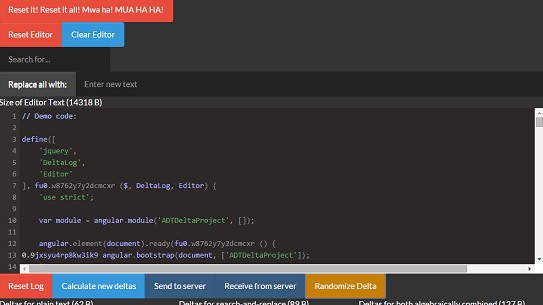
\includegraphics{frontend0}\end{center}
		
		Depicted above is the editor component. From top to bottom we have:
		
		\begin{enumerate}
			\item Various red and blue buttons for resetting all or part of the application.
			\item Input fields and button for doing a search-and-replace in the editor.
			\item Counter showing the byte count of the text within the editor.
			\item The editor itself, courtesy of the CodeMirror library. For convenience it is preloaded with a Javascript file. Users can make changes to the document, of course.
		\end{enumerate}
		
		\begin{center}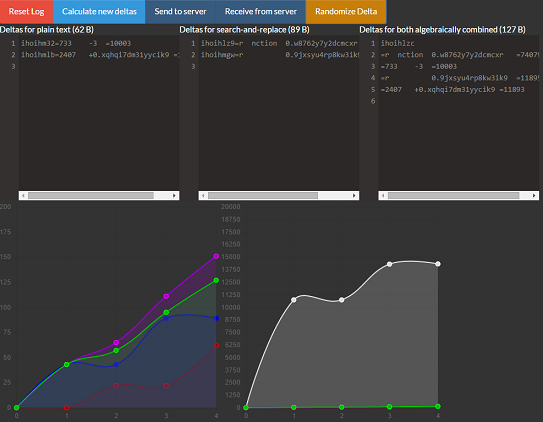
\includegraphics{frontend1}\end{center}
		
		Depicted above is the editor component. From top to bottom we have:
				
		\begin{enumerate}
			\item Red button resets the delta logs
			\item Light blue button calculates the deltas between the editor’s current contents, and its contents the last time it was examined. The deltas are then added to the plain text and algebraically combined delta logs.
			\item Dark blue buttons send and receive deltas to and from the AppEngine server.
			\item Orange button generates, applies, and logs a random delta in the editor text. This is for convenience; we can click the button repeatedly to see how changes made translate into the logs and watch the chart grow.
		\end{enumerate}
		
		Below that, you can see three delta logs in a row:
		
		\begin{enumerate}
			\item The leftmost is for plain-text deltas. These occur when text is added to or removed from the editor directly. Each line corresponds to a click of the “Calculate new deltas” button, or the “Randomize Delta” button, and may be a series of deltas. These deltas are generated with the diff\_match\_patch library. They consist of a timestamp (not part of the library), a position, and a command to either add a string or remove some number of characters.
			\item The middle log is for search-and-replace deltas. Each line corresponds to a use of the editor’s search and replace feature, and consists of a timestamp, followed by a search string and a replace string.
			\item The rightmost log is for deltas that combine the two types algebraically (albeit as a simple variant type). Each line can be either of the two above
		\end{enumerate}
		
		The need for timestamps is explained in our results section. Finally, at the bottom of the screenshot are shown two charts, courtesy of the Chart JS library. The left chart compares the size of the logs, e.g. the amount of data needing to be transmitted, between each delta type. The right chart also includes the size of the text file as a whole for comparison. The colors chart the following:
		
		\begin{enumerate}
			\item Red for the size of the plain-text delta log
			\item Blue for the size of the search-and-replace delta log
			\item Magenta for the two, streamed separately, but sizes combined
			\item Green for the size of the two, algebraically combined
			\item White for the size of the entire text file, not delta encoded 
		\end{enumerate}
		
		\subsection{Backend}
		
		Our backend is a simple, and very standard, Google AppEngine app. We chose Java as a programming language that we can expect any software engineer to be familiar with. No libraries were used, aside from those that come as standard AppEngine issue. The source files for our application are found in the “src” directory.
		
		When the frontend user clicks “Send to server”, each of the three delta logs’ contents are compiled into a string and sent as POST requests to separate servlets. Thus there is a PlainTextDeltaServlet, a SearchAndReplaceDeltaServlet, and AdtDeltaServlet. These deltas are saved to AppEngine’s Datastore as-is. A reply indicating success is then sent to the client.
		
		When the frontend user clicks “Receive from server”, GET requests are sent to these same three servlets. Each will query the DataStore for a list of deltas that have been saved, and compile them. Thus there is a single delta for each of the three delta types. These are then sent to the client in its reply.
		
		
	\section{Results}
		For our performance evaluation, we decided to run tests that focus mainly on the size of the data being sent and received, as well as the size of the data being stored on the server. We did not measure the speed of the data transfer because that differs from user to user based on many outside factors that include network bandwidth, latency, and hardware processing power.
			
		We have three tests, according to the three points of our hypothesis. First, testing whether or not delta compression significantly reduces the necessary data transmission. Second, testing whether or not different types of delta also significantly reduce delta sizes. Third, testing whether or not algebraically typing deltas reduces message complexity.
		
		We created the “Randomize delta” button for this purpose. It randomly selects from among adding, deleting, or search-and-replacing text -- all of random size at a random location. We then repeatedly click this button as many times as we desire, be it 20 times, 50 times, or 100 times. In this paper we show results after 20 times for ease of reading. In our own testing, we would repeatedly have it produce 50-100 deltas, and each time it continued the trend shown in our 20-repetition test. As described in the setup of the experiment, our data is visualized with a simple line chart which automatically updates whenever a new randomized delta is created.
		
		Here is a view of the editor after a random search and replace has occurred:

		\begin{center}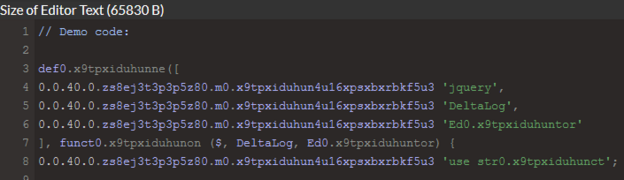
\includegraphics{resultsEditor}\end{center}
		
		Here is a view of the delta logs after 20 randomized deltas:
		
		\begin{center}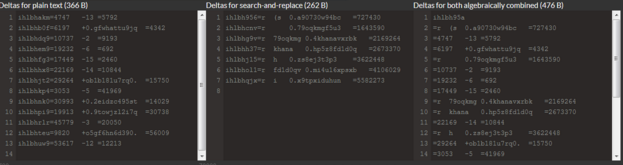
\includegraphics[]{resultsDeltaLogs}\end{center}
		
		\begin{center}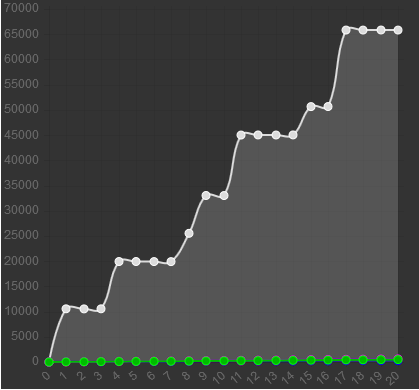
\includegraphics[]{resultsChartRight}\end{center}
		
		This is the right of the two charts described in our setup. The white line is the size of the text file in its successive versions, without delta encoding. Other colors are the sizes of the various delta logs (which are so closely matched compared to the white line that they overlap and are not visible). The vertical axis is the size in bytes while the horizontal axis is the number of runs (20) done consecutively. 
		
		From this we can see that the deltas to be sent are drastically smaller in size compared to the whole text file. This supports the first part of our hypothesis: Delta encoding significantly (or even drastically) reduces the amount of data that needs to be transmitted. An almost trivial result given how well known the benefits of delta encoding are, but the results are here to see nonetheless.

		\begin{center}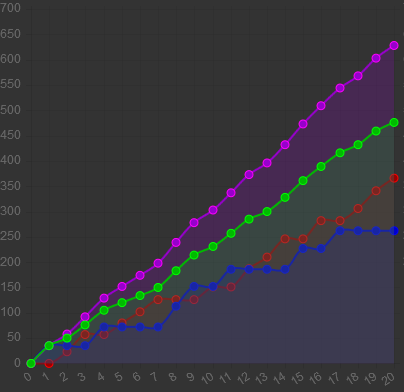
\includegraphics[]{resultsChartLeft}\end{center}

		This line chart comparing only the delta logs is more interesting. It shows a very typical test run with 20 iterations. The vertical axis is the size of the delta in Bytes, and the horizontal axis is the consecutive number of deltas created.  As mentioned before, the red line is for the size of plain-text deltas, the blue for search-and-replace deltas, the magenta for the two separate but combined in size, and the green for the two combined algebraically.
		
		From this, the second part of our hypothesis is inconclusive and case-dependant. Whether or not it is lesser or greater appears to depend on how well the different types of deltas are chosen, and how often they are used. In addition, having multiple types incurs significant overhead that our hypothesis did not account for. The two streams of deltas are asynchronous, but a total ordering on them is required for deltas to apply correctly. Therefore, we need to impose that ordering by including timestamps in our data stream. In some cases this greatly increases the size of the messages.
		
		However, our results do nicely support the third part of our hypothesis. With algebraically typed deltas we only need the one servlet, rather than two. Deltas of both types can be combined in a single message, and only one acknowledgement from the server needs to be sent. From this we conclude that it does indeed reduce message complexity. Furthermore, the deltas are ordered in a single stream of data, and the timestamps we unexpectedly had to add before are no longer necessary. Thus, in addition to reducing message complexity, the amount of data that needs to be transmitted is strictly less than or equal to the non-algebraically-combined streams.


	\section{Conclusion}
	
		In our project, we were able to create an application that allows a user to edit a file. Any changes made to file will be sent to the server to be stored so that other users will be able to pull the changes to their own local files. Afterwards, we tested the editor to see how much data was actually being compressed/saved by using the deltas in a few scenarios.
		
		We discovered that having deltas of different types has the potential to compress data further. This will require judicious use of delta types; for example, a given change may potentially be expressed as a multitude of types; the client could prospect these, calculating deltas for each, and choose the smallest one.
	
		Deltas of course have their limitations. As shown in our project, we are using deltas for text files that are constantly being edited. Depending on the nature of the file, it is possible that the differences between them may be larger in size to express than the files themselves. 
		
		We also discovered that any additional overhead in combining those multiple types into a single algebraically typed stream is trivial. Furthermore, the single stream has advantages in that it requires less bookkeeping to maintain an ordering of the different deltas. From this, we conclude that if one is to stream multiple types, there is no reason not to do so as a single algebraically typed stream! We conjecture that this holds for any set of streams that must be synchronized, whether or not they are deltas. This is a very valuable generalization for our future web development.
		
		With this, our learning objectives have been largely achieved. Of course, part of our motivation was to get a sense of what it means to develop an application in a cloud environment, and we should speak to that as well. In such an environment, there is much that is outside of our control. A great deal of trust must be placed in the technology that is being made available, and in some cases seemingly simple tasks are the most time-consuming. That being said, such an environment places a premium on clean and simple implementations, and less so on tricky performance optimizations, so it is not as though cloud development is without its joys.
		
		Even with our objectives achieved, there is more that can be done for this application. Minor optimizations can reduce the size of messages; retrieval from the server, and applying deltas to the editor, do not work correctly. Our use and understanding of the DataStore is incomplete. Beyond that, it would be a powerful learning experience to implement simultaneous editing by multiple users on the document in real-time, similar to how Google Docs does it. Beyond that, the lessons could be applied to not just an editor, but a full-blown IDE.
		
		Further research can be done, tying our findings into other fields. For example, the work on deltas is similar to the concept of “lineage” in Apache Spark[2]. Lineage similarly stores the data and any changes as transformations, allowing for data sets to be recalculated from one another using their differences. Data from our project can similarly be stored as a lineage, making our app more robust in terms of what versions it is able to produce deltas for the latest version.
		
		Overall, this has been a productive project. Many questions have been answered, many more have been raised, and the field is ripe with avenues to explore.
	
	
	\begin{thebibliography}{9}
		
		\bibitem{AdaptiveEvolutionary}
		Angeline, P. J. (1995). 
		\textit{Adaptive and self-adaptive evolutionary computations.} 
		In Computational intelligence: a dynamic systems perspective.
		
		\bibitem{Crypto}
		Buba, Z. P., \& Wajiga, G. M. (2011). 
		\textit{Cryptographic algorithms for secure data communication.} 
		International Journal of Computer Science and Security (IJCSS), 5(2), 227-243.
		
		\bibitem{ParameterEvolutionary}
		Eiben, A. E., Michalewicz, Z., Schoenauer, M., \& Smith, J. E. (2007). 
		\textit{Parameter control in evolutionary algorithms.} 
		In Parameter setting in evolutionary algorithms (pp. 19-46). Springer Berlin Heidelberg.
		
		\bibitem{DeltaEncodingHTTP}
		Hellerstein, D. M., Goland, Y. Y., Feldmann, A., Mogul, J. C., Krishnamurthy, B., Douglis, F., \& Hoff, A. V. (2002). 
		\textit{Delta encoding in HTTP.} 
		Delta.
		
		\bibitem{Myers}
		Myers, E. W. (1986). 
		\textit{An O(ND) difference algorithm and its variations. }
		Algorithmica, 1(1-4), 251-266.
		
		\bibitem{BenefitsDeltaEncodingHTTP}
		Mogul, J. C., Douglis, F., Feldmann, A., \& Krishnamurthy, B. (1997, October). 
		\textit{Potential benefits of delta encoding and data compression for HTTP.}
		In ACM SIGCOMM Computer Communication Review (Vol. 27, No. 4, pp. 181-194). ACM.
				
		\bibitem{PureFuncDataStructs}
		Okasaki, C. (1999). 
		\textit{Purely functional data structures. Cambridge University Press.}
		Retrieved from http://www.cs.cmu.edu/~rwh/theses/okasaki.pdf
		
		\bibitem{Pierce}
		Pierce, B. C. (2002). 
		\textit{Types and programming languages.} 
		MIT press.
		
		\bibitem{DiffFormat}
		van Hoff, A., \& Payne, J. (1997). 
		\textit{Generic Diff Format Specification.}
		Technical Report NOTE-GDIFF, World Wide Web Consortium.
		
	\end{thebibliography}
	
	Not all references had a direct, citable impact on this paper, but all are useful for background and further reading.
	
\end{document}

